\documentclass{article}
\usepackage[en]{ukon-infie}
\usepackage[utf8]{inputenc}
\usepackage{algorithm2e}
\usepackage{amsmath}
\usepackage{graphicx}
% kann de oder en sein
% kann bubble break, topexercise sein

\Names{Jonas Probst, Simon Giebenhain, Gabriel Scheibler, Clemens Gutknecht}
\Lecture[DLCV]{Deep Learning for Computer Vision}
\Term{WS 2017/18}

\begin{document}
    \begin{ukon-infie}[18.2.18]{5}

		
		\begin{exercise}[p=50+10]{action recognition in video sequences using LSTM}
		\question{}
		{
		The source code for our LSTM architecture can be found in \textbf{lstm.py}.\\
		Our architecure is based on the example linked on the exercise sheet. Furthermore we added 2 convolutional layers and one fully connected layer between the input images and the lstm. Therefore the input into the lstm were the linearized feature maps of dimensions $16 \times 7$ with depth$16$. \\
		Additionally we applied dropout the output of the LSTM-net to tackle overfitting a little bit.\\
		We trained with 70 sequences and tested with the remaining 5. Due to the small training and test sets, overfitting was quite strong and the test accuracy strongly depended on the random selection of the 5 test images. Also this might be the reason, why the test accuracy jumps wildly around.\\
		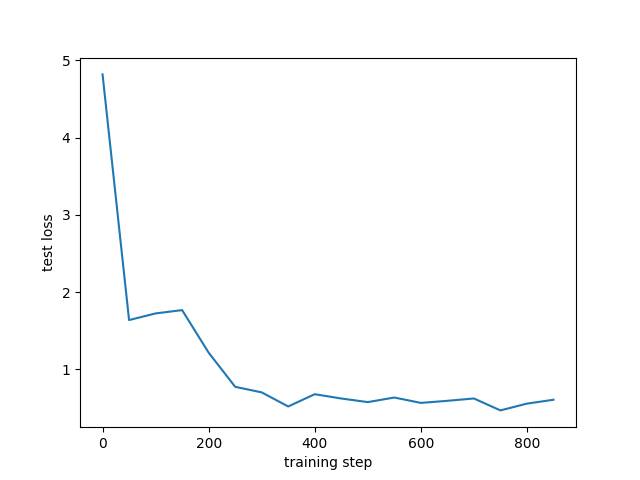
\includegraphics[scale=0.4]{lstm_test_loss.png}
		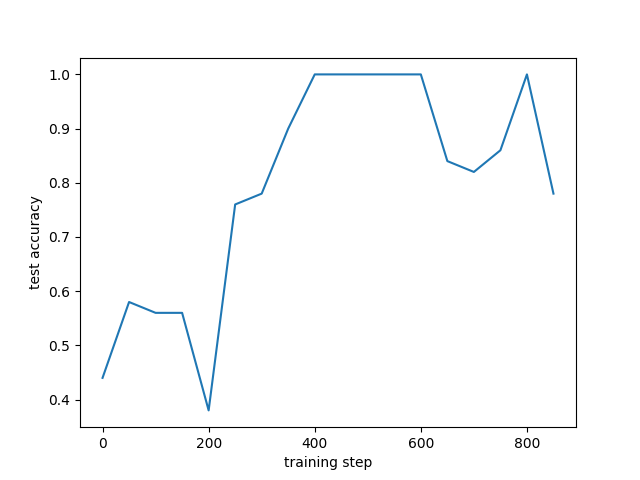
\includegraphics[scale=0.4]{lstm_test_accuracy.png}		
		}
		\question{}
		{
		In order to save computational capacities, we reduced the training steps for the 5-fold cross validation to 1500 steps. \\
		Due to a lack of training examples we didn't have a distinct test set, but calculated the 'test' loss/accuracy by averaging over the validation sets of the 5-folds of the cross validation.\\
		We tested the following number of hidden units to describe the lstm cell states: 25, 100, 225, 400.\\
		The source code can be found in \textbf{cross.py}.\\
		
		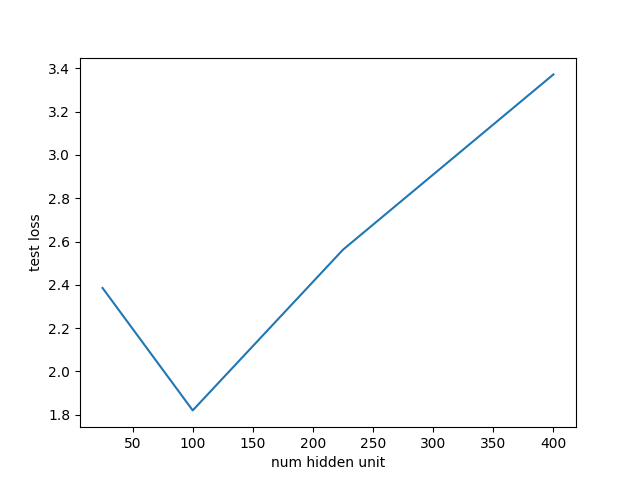
\includegraphics[scale=0.4]{cross_loss.png}
		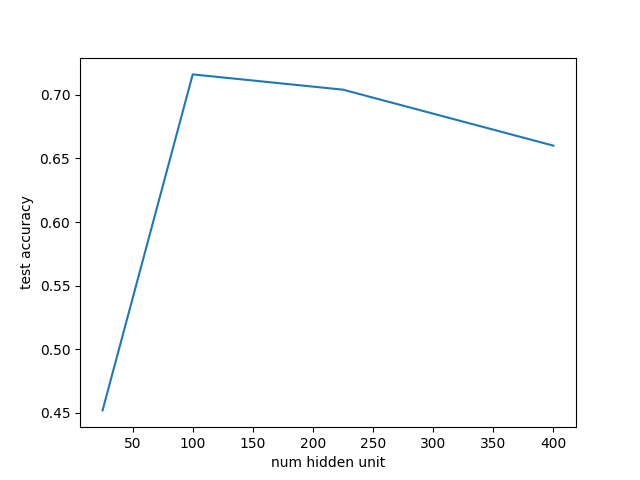
\includegraphics[scale=0.4]{cross_accuracy.png}

		}
		\question{}
		{
		We stiched together the sequences of mixed actions in the following way:\\
		There are 5 actions with frames randomly distributed between 20 and 28 frames. The we cut off all frames after the 100th frame.\\
		The source code can be found in \textbf{seq\_seg.py}\\
		We achieved the following average loss and accuracy for classifying the single frames of the mixed sequences:\\
		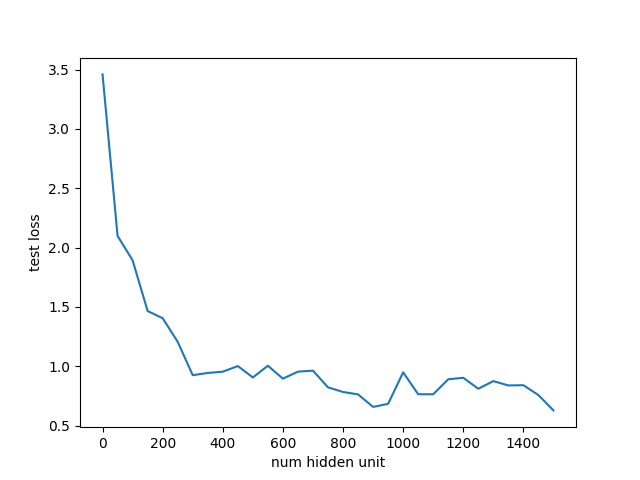
\includegraphics[scale=0.4]{seg_loss.png}
		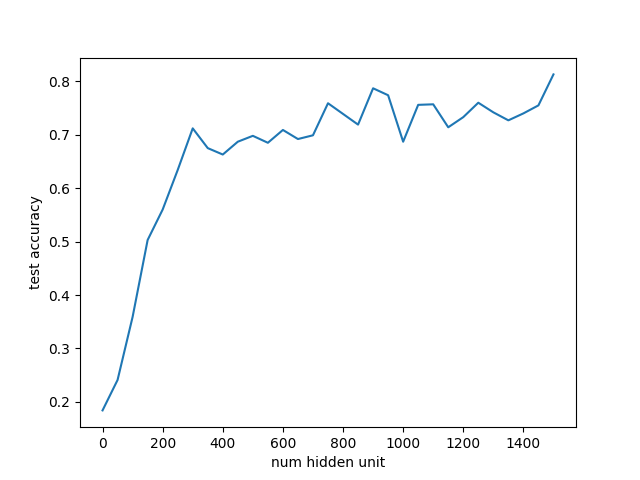
\includegraphics[scale=0.4]{seg_accuracy.png}
		}
		\end{exercise}
		
\end{ukon-infie}
\end{document}